% Options for packages loaded elsewhere
\PassOptionsToPackage{unicode}{hyperref}
\PassOptionsToPackage{hyphens}{url}
%
\documentclass[
]{article}
\usepackage{amsmath,amssymb}
\usepackage{lmodern}
\usepackage{ifxetex,ifluatex}
\ifnum 0\ifxetex 1\fi\ifluatex 1\fi=0 % if pdftex
  \usepackage[T1]{fontenc}
  \usepackage[utf8]{inputenc}
  \usepackage{textcomp} % provide euro and other symbols
\else % if luatex or xetex
  \usepackage{unicode-math}
  \defaultfontfeatures{Scale=MatchLowercase}
  \defaultfontfeatures[\rmfamily]{Ligatures=TeX,Scale=1}
\fi
% Use upquote if available, for straight quotes in verbatim environments
\IfFileExists{upquote.sty}{\usepackage{upquote}}{}
\IfFileExists{microtype.sty}{% use microtype if available
  \usepackage[]{microtype}
  \UseMicrotypeSet[protrusion]{basicmath} % disable protrusion for tt fonts
}{}
\makeatletter
\@ifundefined{KOMAClassName}{% if non-KOMA class
  \IfFileExists{parskip.sty}{%
    \usepackage{parskip}
  }{% else
    \setlength{\parindent}{0pt}
    \setlength{\parskip}{6pt plus 2pt minus 1pt}}
}{% if KOMA class
  \KOMAoptions{parskip=half}}
\makeatother
\usepackage{xcolor}
\IfFileExists{xurl.sty}{\usepackage{xurl}}{} % add URL line breaks if available
\IfFileExists{bookmark.sty}{\usepackage{bookmark}}{\usepackage{hyperref}}
\hypersetup{
  pdftitle={Assignment 2: Two competing species},
  hidelinks,
  pdfcreator={LaTeX via pandoc}}
\urlstyle{same} % disable monospaced font for URLs
\usepackage[margin=1in]{geometry}
\usepackage{graphicx}
\makeatletter
\def\maxwidth{\ifdim\Gin@nat@width>\linewidth\linewidth\else\Gin@nat@width\fi}
\def\maxheight{\ifdim\Gin@nat@height>\textheight\textheight\else\Gin@nat@height\fi}
\makeatother
% Scale images if necessary, so that they will not overflow the page
% margins by default, and it is still possible to overwrite the defaults
% using explicit options in \includegraphics[width, height, ...]{}
\setkeys{Gin}{width=\maxwidth,height=\maxheight,keepaspectratio}
% Set default figure placement to htbp
\makeatletter
\def\fps@figure{htbp}
\makeatother
\setlength{\emergencystretch}{3em} % prevent overfull lines
\providecommand{\tightlist}{%
  \setlength{\itemsep}{0pt}\setlength{\parskip}{0pt}}
\setcounter{secnumdepth}{-\maxdimen} % remove section numbering
\ifluatex
  \usepackage{selnolig}  % disable illegal ligatures
\fi

\title{Assignment 2: Two competing species}
\author{}
\date{\vspace{-2.5em}}

\begin{document}
\maketitle

\hypertarget{stability-of-one-species-equilibirum}{%
\subsection{1. Stability of one-species
equilibirum}\label{stability-of-one-species-equilibirum}}

\emph{In examining the dimensionless Lotka-Volterra competition model in
class, we saw that for} \(u^∗_1 = 1, u^∗_2 = 0\) \emph{to be stable, we
needed} \(\alpha_{21} > 1\). \emph{Interpret and justify this result.}
\emph{Would your conclusions be affected if you learned that}
\(\alpha_{12}\) \emph{were extremely large?}

\(\alpha_{21}\) is the effect of species 1 on species 2. If it is
smaller than 1, that means that the presence of species 1 will allow for
more growth in species 2 when it invades. This means the equilibrium of
only species 1 is unstable. This is still true when \(\alpha_{12}\), the
effect of species 2 on species one is large. Because this effect is
negative, it would even speed up the replacement of species 1.

\hypertarget{invasion-analysis}{%
\subsection{2. Invasion Analysis}\label{invasion-analysis}}

\[\left. \frac{dN_1}{dt}\right. |_{N_1=0,N_2=N_2^*}>0\] We look at the
equation for \(\frac{dN_1}{dt}\) when \(N_1\) is very very small
\[\frac{dN_1}{dt}= r_1N_1(1-\frac{N_1}{K_1}-b_{1,2}\frac{N^*_2}{K_1})\]
\(rN_1\) is going to be very small but positive when \(N_1\) invades so
we search for an expression where
\((1-\frac{N_1}{K_1}-b_{1,2}\frac{N_2}{K_1})>0\). Since
\(\frac{N_1}{K_1}\) is very small, everything depends on
\(b_{1,2}\frac{N_2^*}{K_1}<1\). This is the case when
\(b_{1,2}N_2^*<K_1\). Put biologically, the negative effect of species 2
on species 1 at species 2's equilibrium \(b_{1,2}N_2\) needs to be
smaller than the carrying capacity of \(K_1\). This makes sense
intuitively since in order to invade while \(N_2\) is at equilibirum
there needs to be some empty space in the niche that \(N_1\) would
occupy and part of which it shares with \(N_2\). This ties in with the
traditional few of competition as a description of the niche overlap of
two species. The term \(b_{1,2}\frac{N_2^*}{K_1}\) is the same as
\(a_{1,2}\) in our substitution. Comparing invasibility analysis to
stability analysis, we see they are very similar, both setting one
species to its equilibirum and introducing change in the other. The
difference is that invasibility always means the second species starts
at 0, while stability analysis can mean the other species can be at any
equilibrium and undergo a small change in population.

\hypertarget{equilibria-and-their-stability}{%
\subsection{3. Equilibria and their
Stability}\label{equilibria-and-their-stability}}

\[ \frac{dx}{dt}=x(24-x-2y)\] \[ \frac{dy}{dt} = y(30-y-2x)\] We solve
to find the equilibria: \[
\begin{cases} 
x^*= 0 \\
y^*= 0
\end{cases}
\begin{cases} 
x^*= 0 \\
y^*= 30
\end{cases}\begin{cases} 
x^*= 24 \\
y^*= 0
\end{cases}
\begin{cases} 
x^*= 12 \\
y^*= 6
\end{cases}
\] We can see that of the four equilibria only \(x^*= 12 y^*= 6\) is
feasible since \(x>0\) and \(y>0\). Next we evaluate all four points for
stability using the Jacobian matrix of the system. \[
\mathbf{J} = 
\begin{bmatrix}
\displaystyle \frac{\partial f_1}{\partial u_1} & \displaystyle \frac{\partial f_1}{\partial u_2}\\
\displaystyle \frac{\partial f_2}{\partial u_1} & \displaystyle \frac{\partial f_2}{\partial u_2}
\end{bmatrix} = 
\begin{bmatrix}
24-2x-2y & -2x \\ 
-2y & 30-2y-2x
\end{bmatrix}
\] From here we check whether \(Det(\mathbf{J})>0\) and
\(Tr(\mathbf{J})<0\) for each potential eqilibrium.

For \(x^*=y^*=0\) \[
\mathbf{A} = 
\begin{bmatrix}
24 & 0 \\ 
0 & 30
\end{bmatrix}
\] Thus the characteristic polynomial is \[
(24-\lambda)(30-\lambda) \rightarrow \lambda_1 = 30, \lambda_2 =24
\]

This means \(Tr(\mathbf{A})>0\) and the equilibrium is unstable
(remember
\(Tr(\mathbf{J})=\lambda_1+\lambda_2)\),\(Det(\mathbf{J}) =\lambda_1\times\lambda_2\))

For the second candidate \(x^*= 0, y^*= 30\), \[
\mathbf{A}= 
\begin{bmatrix}
-36 & 0 \\ 
-60 & -30
\end{bmatrix}\\
(-36-\lambda)(-30-\lambda)+60 = \lambda^2+66\lambda+1140
= \lambda^2 -Tr(\mathbf{A})\lambda + Det(\mathbf{A})\\
 \rightarrow \lambda_1=-36,\quad \lambda_2=-30
\] Thus, \(Tr(\mathbf{A})=-66<0\) and \(Det(\mathbf{A})=1140\) and the
equilibrium is stable.

For the third candidate \(x^*= 24, y^*= 0\) \[
\mathbf{A}= 
\begin{bmatrix}
-24 & -48 \\ 
0 & -18
\end{bmatrix}\\
(-24-\lambda)(-18-\lambda)+48 = \lambda^2+42\lambda+480\\
\rightarrow \lambda_1=-24,\quad \lambda_2=-18
\] This equilibrium is also stable since \(Tr(\mathbf{A})=-42<0\) and
\(Det(\mathbf{A})=1140>0\).

For the fourth equilibirum \(x^*= 12\) and \(y^*= 6\). \[
\mathbf{A}= 
\begin{bmatrix}
-12 & -24 \\ 
-12 & -6
\end{bmatrix}\\
(-12-\lambda)(-6-\lambda)-288 = \lambda^2+18\lambda-260\\
\rightarrow \lambda_1=-3 (3 + \sqrt{33})\approx-26.2337,\quad\lambda_2= 3 (-3 +\sqrt{33})\approx 8.23369
\] Thus, \(Tr(\mathbf{A})=-18<0\), but \(Det(\mathbf{A})=-260<0\) and
the equilibrium is not feasible.

To recap, the single-species equilibria are stable, but both the
no-species and both-species equilibria are unstable. Looking at the
original set of equations we can get an intuition for why this is true,
as the coefficient for the interaction with the other species is larger
than for the interaction with other members of the same species.

To classify our three equilibria, we can look at the Eigenvalues. Any
point where the Eigenvalues have opposite signs is a saddle point, so
this is the case when for the fourth equilibirum when \(x^*= 12\) and
\(y^*= 6\).Depending on which direction the system is perturbed in, it
will drive one of the species to extinction. For the other three
equilibria, \(Det(\mathbf{A})>0\) and the Eigenvalues are real with the
same sign. This means all three are nodes. We can see the dynamics in
the plot below.

\begin{figure}
\centering
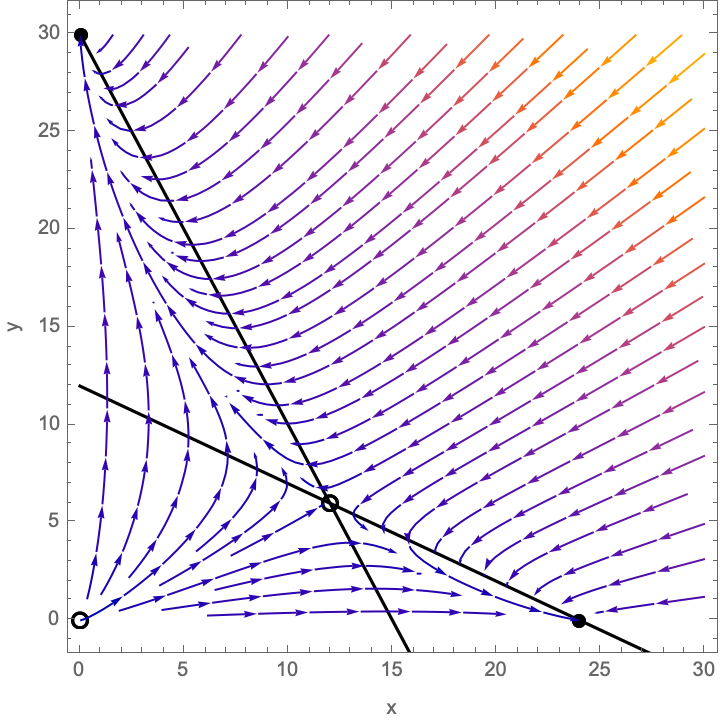
\includegraphics{/Users/katjad/Documents/UChicago/Theoretical Ecology/TheoreticalEcologyCourseGithub/Assignment 2/StreamPlot.png}
\caption{Plot 1: the dynamics of the system shows the four equilibrium
points}
\end{figure}

Code for the plot in Mathematica: Show{[}\{Plot{[}\{(24 - x)/2, -2 (-15
+ x)\}, \{x, 0, 30\}, PlotStyle -\textgreater{} Black, Frame
-\textgreater{} True, FrameLabel -\textgreater{} \{``x'', ``y''\}{]},
ListPlot{[}List /@ \{\{0, 0\}, \{0, 30\}, \{24, 0\}, \{12, 6\}\},
PlotStyle -\textgreater{} Directive{[}Black, PointSize{[}Large{]}{]},
PlotMarkers -\textgreater{} \{\{Graphics{[}Circle{[}{]}{]}, Medium\},
None, None, \{Graphics{[}Circle{[}{]}{]}, Medium\}\}{]},
StreamPlot{[}\{x (24 - x - 2 y), y (30 - y - 2 x)\}, \{x, 0, 30\}, \{y,
0, 30\}{]}\}, PlotRange -\textgreater{} \{\{0, 30\}, \{0, 30\}\},
AspectRatio -\textgreater{} 1{]}

\end{document}
